\chapter{Analysing the properties of Data Models and Query Languages}\label{cha:datadef}

\epigraph{\textit{Therefore a science, the advancement of science, and the acquisition of science, is not simply the oblivion of old [scientific] prejudices, or the fall of certain obstacles [to understanding], it is a new grid [of concepts] that masks certain things while allowing for the appearance of new knowledge}.}{--- Michel Foucault on \textit{The Chomsky-Foucault Debate: On Human Nature}, (1971)}

The previous chapter aimed to evaluate present data structures and query languages within the context of data integration. Bearing such considerations in mind, we analyse currently-proposed data models and query languages: as a result, we have that current data models do not support structural aggregation and that current query languages cannot handle both data and schema at the same time. Both these features are required within data integration scenarios. Moreover, in this chapter we also compare the previous data model with the property graph data model and its extensions. We draw the following conclusions:
\begin{itemize}
\item The relational data model (Section \ref{sec:relationalcmp}) does not distinguish entities from relationships (\textit{semantic overloading}), and does not represent data and data properties ($M$, $MM$) within the same representation (Section \ref{subsec:dmalgebra}).
\item Semistructured data provide a multimap association between properties and values (e.g., multiple \textit{tags} with the same name); even if both semistructured and nested relational model allow a content-container relation, only the stream data model meets the requirements for  structural aggregation (Section \ref{sec:semistructured}).
\item Current graph data model distinguish entities from relationships, but do not provide a structural aggregation over both vertices and edges (Section \ref{sec:datamodelglit}).
\end{itemize}


For each data model we'll also briefly discuss their query languages and their implications with respect to the data manipulation abilities. In particular, we're going to analyse graph query languages' features with respect to their underlying data models (Section \ref{sec:dbqlang}).
\begin{figure}[!pth]
	%\begin{adjustbox}{max width=\textwidth}
	\begin{minipage}[b]{\textwidth}
		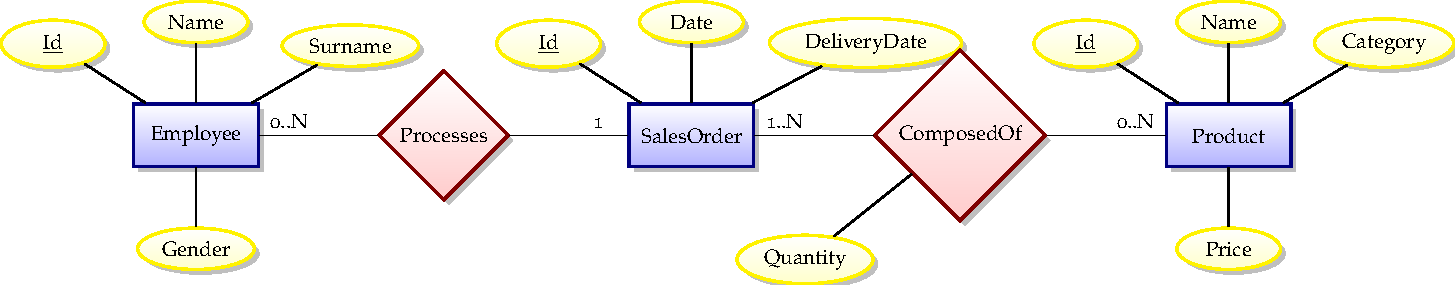
\includegraphics[scale=.6]{fig/02models/01erschema}
		\subcaption{Representing the ER model for a subset of a enterprise database, describing that each employee is able to create sales order formed by at least one product. }
		\label{fig:erschema}
	\end{minipage}\quad

	\begin{minipage}[b]{\textwidth}
		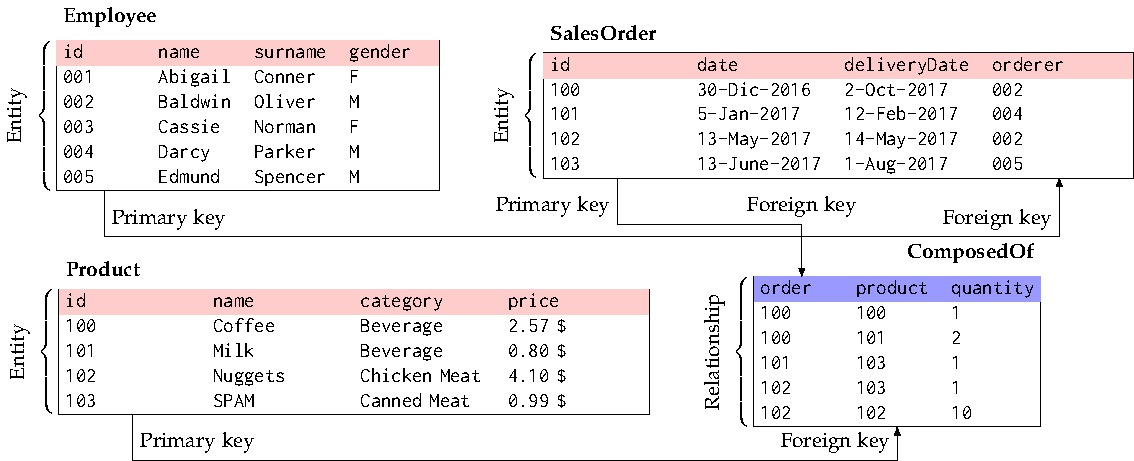
\includegraphics[scale=.7]{fig/02models/02instance}
		\subcaption{An instance of the overlying ER model. Some relations are directly expressed with Primary Key-Foreign Key relations (\textbf{Processes}), while others (\textbf{ComposedBy}) are require an intermediate table. The name of the relations appear on top of each table.}
		\label{fig:instance}
	\end{minipage}

	\begin{minipage}[b]{\textwidth}
		\centering
		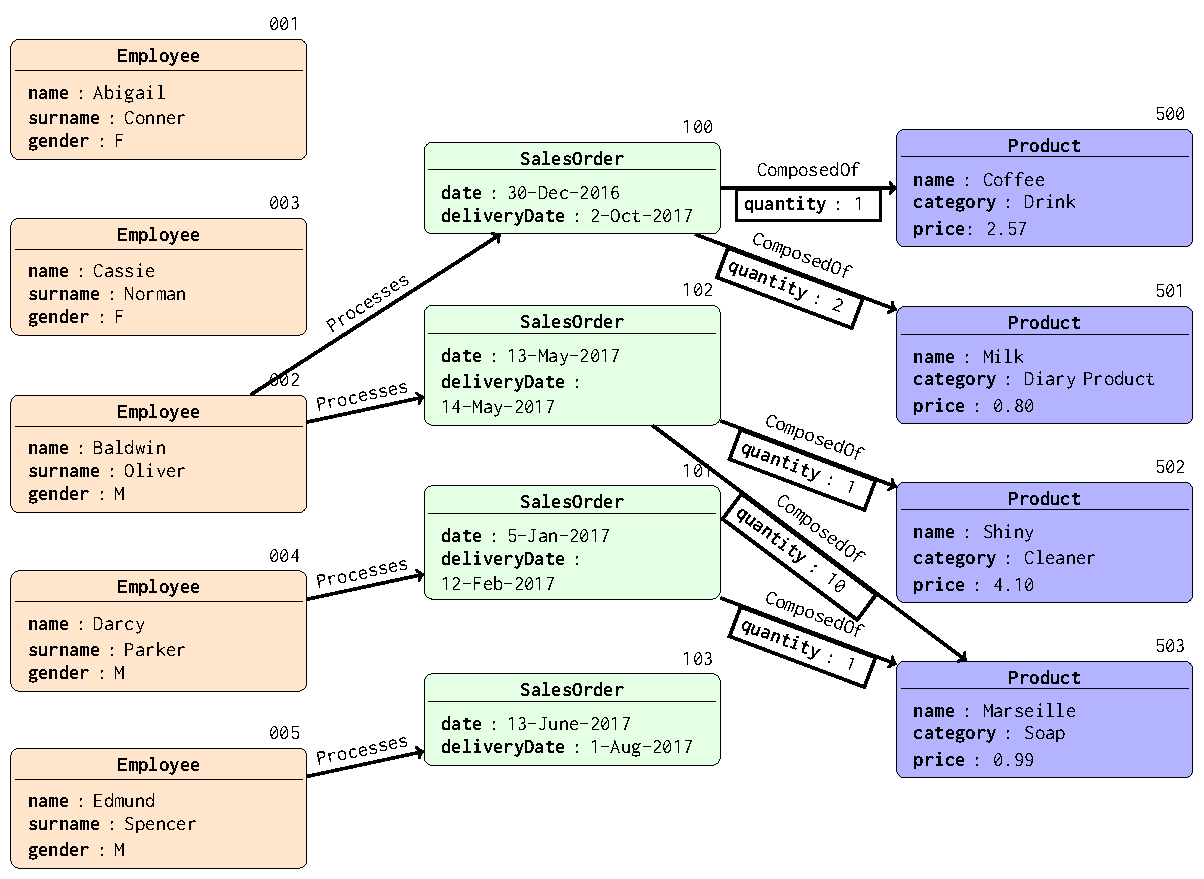
\includegraphics[scale=.6]{fig/02models/03dbasgraph}
		\subcaption{Representing the same relational database through a property graph. Please note that this is a faithful representation of the ER schema. The association between vertex and edge id's and their property-value association is described in Section \vref{sec:objid} (\textit{Object Identity})}
		\label{fig:graphofdb1}
	\end{minipage}
	%\end{adjustbox}
	\caption{While the process of modelling a relational database (\subref{fig:erschema}) requires to distinguish between entities and relationships, its instantiation in a logical database model discards them (\subref{fig:instance}). This information could be preserved within the property graph model (\subref{fig:graphofdb1}). }
	\label{fig:relationalinstance}
\end{figure}

